
\section{\uppercase{Signal Quantization For Rapid Classification}}
\label{sec:quantization}

%We are interested in minimizing computational expense of classifying mental gestures. This study investigates a signal quantization technique that reduces the size of EEG data for fast classification but retains high accuracy.

\noindent Our objective is to maximize the accuracy of the classifier while minimizing its computational expense. One way to reduce the computational requirements of a classifier is to reduce the size of the feature vectors on which it is trained and tested. We propose a signal quantization method that allows us to directly adjust the size of feature vectors. Since vector size directly impacts the runtime of the classifier, this technique operationalizes the tradeoff between computational speed and accuracy.

%Generally, we seek to maximize our system's classification accuracy while minimizing its computational expense. One way to reduce the computational requirements of a SVM classifier is to reduce the size of the feature vectors on which it is trained and tested. Our signal quantization method allows us to directly adjust the size of feature vectors by changing the signal's resolution (see 3.1), though lowering the resolution of feature vectors could negatively effect the classifier's performance.

%\subsection{Compressing power spectra in the temporal dimension}

We average the power spectrum time series in the temporal dimension and compute a discrete probability density function (pdf) from the resulting power spectrum in which each component is the mean of its corresponding frequency components through time. This results in a discrete pdf with 1024 components
for each trial, which can be quantized as described in the following section.

%First, we compute an average of all the power spectra associated with a recording. We obtain a discrete probability density function (PDF) in which each bin is the mean of its corresponding bins through time. At this stage, we have a discrete PDF of 1024 bins for the entire n second recording. 

\subsection{Logarithmic Binning}

Since EEG activity is associated with frequencies from 1-40Hz, it is generally presumed that this range contains the majority of relevant signal. However, this frequency range can be polluted with non-neural signals \cite{ball2009signal}, and we do not rule out the possibility that useful signal exists outside this frequency range as well. Muscular activity, for example, might be correlated with mental gestures in some cases. In order to exploit the entire frequency spectrum while preserving our bias toward known sources of useful signal, we select log-spaced data bins through the logarithm of the frequency range. Figure \ref{binnedEEGpowerspec} shows an example of logarithmic binning with 65 bins. The original, 1024-point pdf is compressed more than 10 times, but its original structure is well-preserved.

Data binning offers a simple way to quantize the information contained in the full signal. By taking the mean of several adjacent points in the pdf, we are left with a single bin that represents the local area of spectrum. For example, four contiguous frequencies (1Hz, 1.25Hz, 1.5Hz, 1.75Hz) of the values (4, 4, 5, 5) average into a single bin with the value 4.5. The number of bins can be adjusted to produce feature vectors of different sizes. This vector, which highlights the statistical properties of the power spectrum for each mental task, can be used as an input of variable size to the classifier.

\begin{figure}[!h]
  \vspace{-0.2cm}
  \centering
  {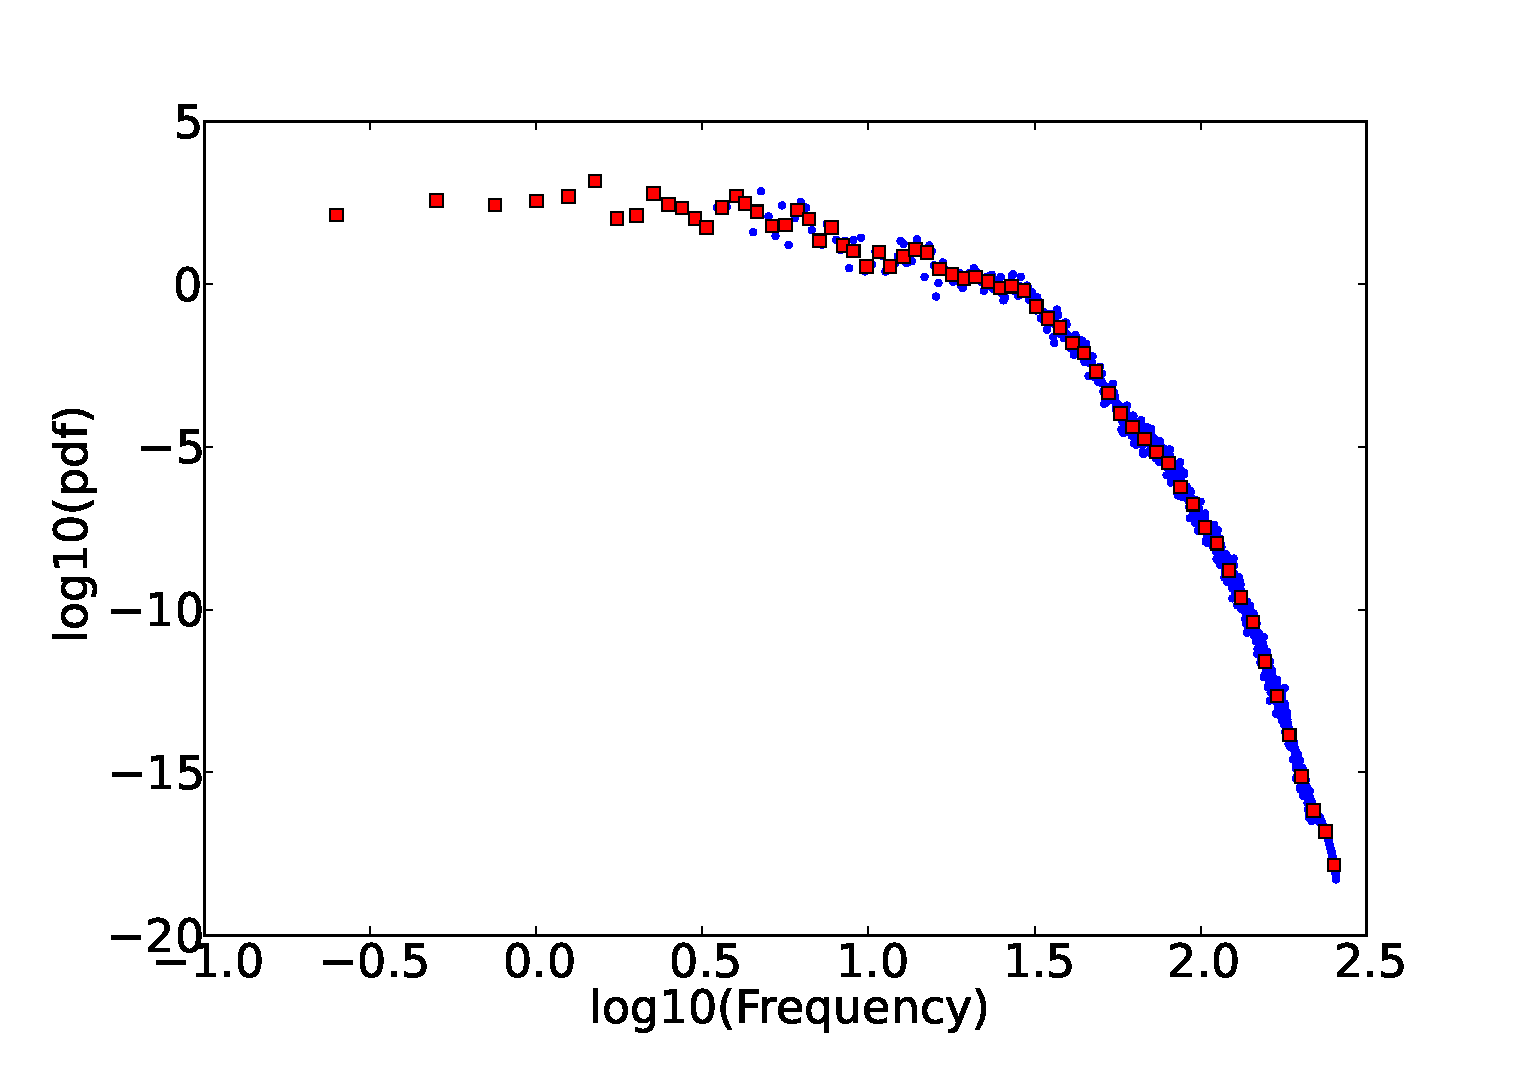
\epsfig{file = Figures/figure1.eps, width = 8cm}}
\caption{In double logarithmic scale, the original 1024 bins (blue dots) of the probability density function (pdf) obtained from averaging the \emph{n} power spectra of one recording, and the resulting quantized pdf with a resolution of 65 log-bins (red). The quantized pdf preserves very well the structure of the original, 1024-point pdf. }
\label{binnedEEGpowerspec}
\vspace{-0.1cm}
\end{figure}

%In summary, we build a probability density function of frequencies captured by the EEG scanning device from all the power spectra in a recording. We then use logarithmically-spaced bins to reduce the original 1024 frequency values to a smaller number of bins (e.g., 100 log-bins in \ref{binnedEEGpowerspec}). This method produces a statistical average of a time series, compressed into a single feature vector that it is easy to use in a classifier.


\subsection{Binary BCI Classifier}

To test the performance of the quantization method, we build a binary BCI using a support vector machine (SVM) classifier, which we train individually on each subject's recordings while varying the bin size. We use LinearSVC \cite{fan_liblinear:_2008}, a wrapper for LibLinear exposed in Python through the scikit-learn library \cite{pedregosa_scikit-learn:_2011}. We chose LinearSVC because BCI classification problems are generally presumed to be linear  \cite{garrett_comparison_2003,lotte_review_2007}, and because LibLinear's underlying C implementation boasts among the fastest train- and test-time performance among state-of-the-art solutions \cite{fan_liblinear:_2008}. We use a hyperparameter of 100, found through a grid-search of a randomly-selected sample of our dataset. We use scikit-learn's built-in cross-validation toolkit, which performs seven cross-validation steps utilizing different splits of data in each round.

Out of the seven mental gestures in the dataset, we want to identify and select, for each individual subject, the two gestures (or \textit{classes}) that we can most reliably differentiate from one another. This results in a personalized, binary classifier, where the SVM can discriminate between two mental gestures performed by the subject with the highest classification accuracy. The gesture pairs may vary from subject to subject. For example, one subject's best-case pair may be \textit{song} and \textit{sport} while another's may be \textit{color} and \textit{finger}. Subjects can then select one of two options by performing one of the mental gestures in their gesture pair.
